\documentclass[11pt,a4paper]{article}

% Packages
\usepackage[utf8]{inputenc}
\usepackage[T1]{fontenc}
\usepackage{lmodern}
\usepackage[margin=1in]{geometry}
\usepackage{graphicx}
\usepackage{xcolor}
\usepackage{hyperref}
\usepackage{enumitem}
\usepackage{fancyhdr}
\usepackage{tikz}
\usepackage{fontawesome5}
\usepackage{tcolorbox}
\usepackage{tabularx}
\usepackage{booktabs}

% Colors
\definecolor{primary}{HTML}{4F46E5}
\definecolor{secondary}{HTML}{6366F1}
\definecolor{accent}{HTML}{10B981}
\definecolor{lightbg}{HTML}{F3F4F6}
\definecolor{darktext}{HTML}{1F2937}
\definecolor{graytext}{HTML}{6B7280}

% Hyperlink setup
\hypersetup{
    colorlinks=true,
    linkcolor=primary,
    urlcolor=primary,
    pdfauthor={INFINITEST},
    pdftitle={User Manual - AI Test Generator}
}

% Header/Footer
\pagestyle{fancy}
\fancyhf{}
\fancyhead[L]{\textcolor{graytext}{\small INFINITEST}}
\fancyhead[R]{\textcolor{graytext}{\small User Manual}}
\fancyfoot[C]{\textcolor{graytext}{\small Page \thepage}}
\renewcommand{\headrulewidth}{0.5pt}
\renewcommand{\footrulewidth}{0pt}

% Custom box styles
\tcbset{
    tipbox/.style={
        colback=accent!10,
        colframe=accent,
        fonttitle=\bfseries,
        title={\faLightbulb\ Tip},
        boxrule=1pt,
        arc=3mm,
        left=5pt,
        right=5pt
    },
    notebox/.style={
        colback=primary!10,
        colframe=primary,
        fonttitle=\bfseries,
        title={\faInfoCircle\ Note},
        boxrule=1pt,
        arc=3mm,
        left=5pt,
        right=5pt
    },
    warningbox/.style={
        colback=yellow!10,
        colframe=orange!80!black,
        fonttitle=\bfseries,
        title={\faExclamationTriangle\ Important},
        boxrule=1pt,
        arc=3mm,
        left=5pt,
        right=5pt
    }
}

% Section styling
\usepackage{titlesec}
\titleformat{\section}{\Large\bfseries\color{primary}}{\thesection}{1em}{}
\titleformat{\subsection}{\large\bfseries\color{secondary}}{\thesubsection}{1em}{}

\begin{document}

% Title Page
\begin{titlepage}
    \centering
    \vspace*{2cm}
    
    % Logo
    
\includegraphics[width=0.35\textwidth]{logo.jpeg}
    
    \vspace{0.8cm}
    
    {\Huge\bfseries\textcolor{primary}{INFINITEST}}\\[0.2cm]
    {\small\textcolor{graytext}{\textit{A Mentors Mantra Product}}}
    
    \vspace{1cm}
    
    {\Huge\bfseries\textcolor{darktext}{User Manual}}\\[0.5cm]
    {\Large\textcolor{secondary}{Test Paper Generator}}\\[0.3cm]
    {\large\textcolor{graytext}{For JEE, NEET, Boards \& Olympiad}}
    
    \vspace{2cm}
    
    \begin{tikzpicture}
        \node[fill=lightbg, rounded corners=8pt, inner sep=20pt] {
            \begin{tabular}{cl}
                \faGlobe & \textbf{Website:} \href{https://www.infinitest.tech}{www.infinitest.tech} \\[8pt]
                \faEnvelope & \textbf{Email:} \href{mailto:help@infinitest.tech}{help@infinitest.tech} \\[8pt]
                \faPhone & \textbf{Contact:} Priyanshu: 9821040290 \\[3pt]
                & \hspace{1.35cm} Nikhlesh: 7456942855
            \end{tabular}
        };
    \end{tikzpicture}
    
    \vfill
    
    {\small\textcolor{graytext}{Version 1.0 | January 2026}}
    
\end{titlepage}

% Table of Contents
\tableofcontents
\newpage

% -----------------------------------------------------------
\section{Introduction}
% -----------------------------------------------------------

INFINITEST Test Generator is a powerful tool designed for \textbf{teachers, coaching institutes, and educators} to create professional-quality test papers in seconds.

\subsection{Key Features}

\begin{itemize}[leftmargin=*]
    \item \textcolor{accent}{\faCheckCircle} \textbf{AI-Powered Questions:} Generate unique, high-quality questions using advanced AI
    \item \textcolor{accent}{\faCheckCircle} \textbf{Multiple Subjects:} Physics, Chemistry, Mathematics, and Biology
    \item \textcolor{accent}{\faCheckCircle} \textbf{Multiple Levels:} Boards, JEE Mains, JEE Advanced, NEET, and Olympiad
    \item \textcolor{accent}{\faCheckCircle} \textbf{Difficulty Control:} Easy, Medium, and Hard difficulty options
    \item \textcolor{accent}{\faCheckCircle} \textbf{Professional PDF:} Beautiful LaTeX-formatted test papers with answer keys
    \item \textcolor{accent}{\faCheckCircle} \textbf{MCQ + Numerical:} Mix of multiple choice and numerical type questions
\end{itemize}

\begin{tcolorbox}[notebox]
For JEE Advanced papers, the first 20\% of MCQs are \textbf{Multi-Correct} type (one or more options correct) to match the actual exam pattern.
\end{tcolorbox}

% -----------------------------------------------------------
\section{Getting Started}
% -----------------------------------------------------------

\subsection{Step 1: Create Your Account}

\begin{enumerate}[leftmargin=*]
    \item Visit \textcolor{primary}{\textbf{\href{https://mentors-mantra-test-generator.vercel.app}{mentors-mantra-test-generator.vercel.app}}}
    \item Click on \textbf{"Sign Up"} button
    \item Enter your details:
    \begin{itemize}
        \item Full Name
        \item Email Address
        \item Phone Number (optional)
        \item Password
    \end{itemize}
    \item Click \textbf{"Create Account"}
    \item Check your email for verification link and click to verify
\end{enumerate}

\subsection{Step 2: Login}

\begin{enumerate}[leftmargin=*]
    \item Go to the website
    \item Enter your registered email and password
    \item Click \textbf{"Login"}
    \item You will be redirected to the test generator dashboard
\end{enumerate}

% -----------------------------------------------------------
\section{Generating a Test Paper}
% -----------------------------------------------------------

\subsection{Step 3: Select Subject}

Choose from the available subjects:

\begin{center}
\begin{tabular}{|c|c|c|c|}
\hline
\textbf{\faAtom\ Physics} & \textbf{\faFlask\ Chemistry} & \textbf{\faCalculator\ Maths} & \textbf{\faLeaf\ Biology} \\
\hline
\end{tabular}
\end{center}

\begin{tcolorbox}[tipbox]
\textbf{Auto-Detection Feature:} When you type a topic, the system automatically detects and selects the correct subject!\\
Example: Type "Integration" $\rightarrow$ Maths is auto-selected.
\end{tcolorbox}

\subsection{Step 4: Select Level}

Choose the difficulty level based on target exam:

\begin{center}
\renewcommand{\arraystretch}{1.5}
\begin{tabularx}{\textwidth}{|l|X|}
\hline
\textbf{Level} & \textbf{Description} \\
\hline
\textcolor{green!60!black}{\textbf{Boards}} & Class 11/12 CBSE/State Board level questions \\
\hline
\textcolor{blue}{\textbf{JEE Mains}} & NTA JEE Main pattern, moderate difficulty \\
\hline
\textcolor{purple}{\textbf{JEE Advanced}} & IIT JEE Advanced pattern, includes multi-correct MCQs \\
\hline
\textcolor{orange!80!black}{\textbf{Olympiad}} & Competition level (NSEP, NSEC, RMO, IMO) \\
\hline
\textcolor{pink!80!black}{\textbf{NEET}} & Medical entrance exam pattern (Biology only has MCQs) \\
\hline
\end{tabularx}
\end{center}

\subsection{Step 5: Enter Topic}

Type the specific topic you want questions on.

\textbf{Examples:}
\begin{itemize}[leftmargin=*]
    \item Physics: "Rotation", "Electrostatics", "Wave Optics"
    \item Chemistry: "Chemical Bonding", "Organic Chemistry - Alcohols", "d-Block Elements"
    \item Maths: "Definite Integration", "Probability", "Conic Sections"
    \item Biology: "Cell Biology", "Genetics", "Plant Physiology"
\end{itemize}

\subsection{Step 6: Set Difficulty \& Question Count}

\begin{itemize}[leftmargin=*]
    \item \textbf{Difficulty:} Easy, Medium, or Hard
    \item \textbf{Number of Questions:} 5 to 50 questions
    \item Questions are automatically split into:
    \begin{itemize}
        \item $\sim$80\% MCQs (Multiple Choice Questions)
        \item $\sim$20\% Numerical Type
    \end{itemize}
\end{itemize}

\begin{tcolorbox}[warningbox]
NEET papers contain \textbf{only MCQs} (no numerical questions) to match the actual exam pattern.
\end{tcolorbox}

\subsection{Step 7: Generate \& Download}

\begin{enumerate}[leftmargin=*]
    \item Click the \textbf{"Generate Test Paper"} button
    \item Wait 30-60 seconds while AI generates questions
    \item Once complete, click \textbf{"Download PDF"}
    \item Your test paper is ready!
\end{enumerate}

\begin{tcolorbox}[tipbox]
You can \textbf{cancel generation} anytime by clicking the "Cancel Generation" button that appears during loading.
\end{tcolorbox}

% -----------------------------------------------------------
\section{Understanding Your PDF}
% -----------------------------------------------------------

The generated PDF includes:

\begin{itemize}[leftmargin=*]
    \item \textbf{Header:} Subject, Topic, and Target Level (e.g., "Target: JEE Advanced")
    \item \textbf{Questions Section:} All MCQs and Numerical questions with proper numbering
    \item \textbf{Answer Key:} Complete answer key on a separate page
    \item \textbf{Footer:} Website and contact information
\end{itemize}

\textbf{File Naming:} \texttt{Top\{N\}\_\{Topic\}\_\{Level\}.pdf}\\
Example: \texttt{Top20\_Integration\_JEE\_Mains.pdf}

% -----------------------------------------------------------
\section{Rate Limits}
% -----------------------------------------------------------

\subsection{Free Usage Limits}

\begin{itemize}[leftmargin=*]
    \item \textbf{3 test papers} per day (free tier)
    \item Rate limit resets automatically
    \item Contact us at \textbf{help@infinitest.tech} for higher limits
\end{itemize}

% -----------------------------------------------------------
\section{Tips for Best Results}
% -----------------------------------------------------------

\begin{enumerate}[leftmargin=*]
    \item \textbf{Be Specific with Topics:} "Electrostatics - Gauss Law" works better than just "Electrostatics"
    \item \textbf{Start with Fewer Questions:} Try 10-15 questions first to check quality
    \item \textbf{Match Level to Students:} Use "Boards" for beginners, "JEE Advanced" for advanced batches
    \item \textbf{Check Answer Key:} Always verify answers before distributing to students
    \item \textbf{Combine Topics:} You can use compound topics like "Thermodynamics and Kinetic Theory"
\end{enumerate}

% -----------------------------------------------------------
\section{Troubleshooting}
% -----------------------------------------------------------

\begin{center}
\renewcommand{\arraystretch}{1.5}
\begin{tabularx}{\textwidth}{|l|X|}
\hline
\textbf{Problem} & \textbf{Solution} \\
\hline
Generation taking too long & Wait up to 60 seconds. For larger papers, it may take longer. \\
\hline
Rate limit reached & Wait for the timer to reset, or contact us for higher limits. \\
\hline
Login issues & Try "Forgot Password" or contact support. \\
\hline
PDF not downloading & Check your browser's download settings or try a different browser. \\
\hline
\end{tabularx}
\end{center}

% -----------------------------------------------------------
\section{Contact \& Support}
% -----------------------------------------------------------

\begin{center}
\begin{tikzpicture}
    \node[fill=lightbg, rounded corners=10pt, inner sep=20pt] {
        \begin{tabular}{cl}
            \faGlobe & \textbf{Website:} \href{https://www.infinitest.tech}{www.infinitest.tech} \\[10pt]
            \faEnvelope & \textbf{Email:} \href{mailto:help@infinitest.tech}{help@infinitest.tech} \\[10pt]
            \faTelegram & \textbf{Telegram:} \href{https://t.me/mentorsmantraofficial}{t.me/mentorsmantraofficial} \\[10pt]
            \faPhone & \textbf{Priyanshu:} 9821040290 | \href{mailto:priyanshu@me.iitr.ac.in}{priyanshu@me.iitr.ac.in} \\[5pt]
            \faPhone & \textbf{Nikhlesh:} 7456942855 | \href{mailto:nikhlesh_s@me.iitr.ac.in}{nikhlesh\_s@me.iitr.ac.in}
        \end{tabular}
    };
\end{tikzpicture}
\end{center}

\vspace{1cm}

\begin{center}
\textcolor{graytext}{\rule{0.5\textwidth}{0.5pt}}\\[0.5cm]
\textcolor{graytext}{\small Thank you for choosing INFINITEST!}\\
\textcolor{primary}{\textbf{Empowering Educators, Transforming Education}}
\end{center}

\end{document}
